\chapter{Rotational Dynamics}

\begin{marginfigure}%
  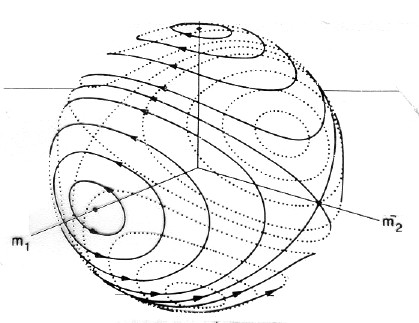
\includegraphics[width=\linewidth]{rigidbody.jpg}
  \caption{Phase portrait of the free rigid body, such as a hammer tossed in the air.}
  \label{fig:marginfig}
\end{marginfigure}


\textit{The Harley's got a little too much torque.}  \\
\noindent\textbf{-   Evel Knievel}


 \section{Rigid Bodies}
 A rigid body is an idealization of a solid body in which deformation is neglected. In other words, the distance between any two given points of a rigid body remains constant in time regardless of external forces exerted on it.  A rigid body is considered to be non-deformable.
 
 \marginnote{Rigidity is a quality found in people and objects that don't bend, though they might eventually break. When we see rigidity in a person, it means they're severe, like a teacher who punishes you for being late even though you were busing saving an orphan from a polar bear.}
 
 
 \section{Torque}
 Torque, moment, or moment of force is the tendency of a force to rotate an object about an axis, fulcrum, or pivot. Just as a force is a push or a pull, a torque can be thought of as a twist to an object. Mathematically, torque is defined as the cross product of the lever-arm distance vector and the force vector, which tends to produce rotation.
  $$\overrightarrow{\tau}\equiv \overrightarrow{r}\times  \overrightarrow{F}$$
  %$$\overrightarrow{\tau}=\lim_{\Delta \rightarrow 0}\frac{\Delta \overrightarrow{l}}{\Delta t}$$
%\vspace{0.1cm}

\section{Newton's First Law for Rigid Bodies}
$$\sum{ \overrightarrow{F}_{ext}}=0 \ \ \longleftrightarrow \ \ \overrightarrow{a}=0 $$
$$\sum{ \overrightarrow{\tau}_{ext}}=0 \ \ \longleftrightarrow \ \ \overrightarrow{\alpha}=0$$ \ \ \ \ \ \marginnote{Torques may be applied around any axis.  Torques, in general, have no meaning without an indication of where they are calculated with respect to.}


 \section{Statics}
 $$\sum{ \overrightarrow{F}_{ext}}=0$$
  $$\sum{ \overrightarrow{\tau}_{ext}}=0$$
  
  \newpage
  
\section{Newton's Second Law for Rigid Bodies}
Newton's second law for rigid bodies related the total torque to the angular acceleration of the system.  The inertial factor serving as the constant of proportionality is the moment of inertia.
$$\sum{ \overrightarrow{F}_{ext}}=m \overrightarrow{a}$$
$$\sum{ \overrightarrow{\tau}_{ext}}=I \overrightarrow{\alpha}$$
 \vspace{0.1cm}
 
 \section{Pure Moments/Couples}
 A pure moment, or couple, is a set of forces which add to zero but are applied in such a way to give a net torque.  In the case of a couple the net torque can be calculated around any point.  Isn't that neat?  Can you prove that mathematically?
 $$\sum{ \overrightarrow{F}_{ext}}=0$$
  $$\sum{ \overrightarrow{\tau}_{ext}}=I \overrightarrow{\alpha}$$
  \vspace{0.1cm}
  
 \section{Moments of Inertia}
 \vspace{0.1cm}
 \marginnote{Our treatment is in 2-D.  The 3-D treatment requires more complicated mathematical representations and is beyond the scope of an introductory course.}
 Consider a rigid body consisting on $N$ massive particles.  We use an index variable $i$ so that each particle has a mass $m_i$ and a position vector $\overrightarrow{r_i}$.  We define the moment of inertia for rotations around the origin as follows.  It is the sum of the masses "weighted" by their square distance from the axis of rotation.
 \vspace{0.1cm}
$$ I\equiv \sum\limits_{i=1}^{N} r_i^2m_i$$
\vspace{0.1cm}
The moment of inertia depends on the rotational axis it is in reference to.  Moving the axis of rotation to the center of mass minimizes the moment of inertia.  We use an $\underbar{underbar}$ to notate this. 
\vspace{0.1cm}
$$ \underbar{I}=\sum\limits_{i=1}^{N} \underbar{r}_i^2m_i$$
%\vspace{1cm}

 \section{Parallel Axis Theorem}
 Moving the axis of rotation a distance $D$ from the center of mass gives a new moment of intertia.
 \vspace{0.1cm}
 $$ I= \underbar{I}+MD^2$$
 
 \newpage
 
 \section{Example Moments of Inertia}
  \vspace{1cm}
  
 \begin{center}
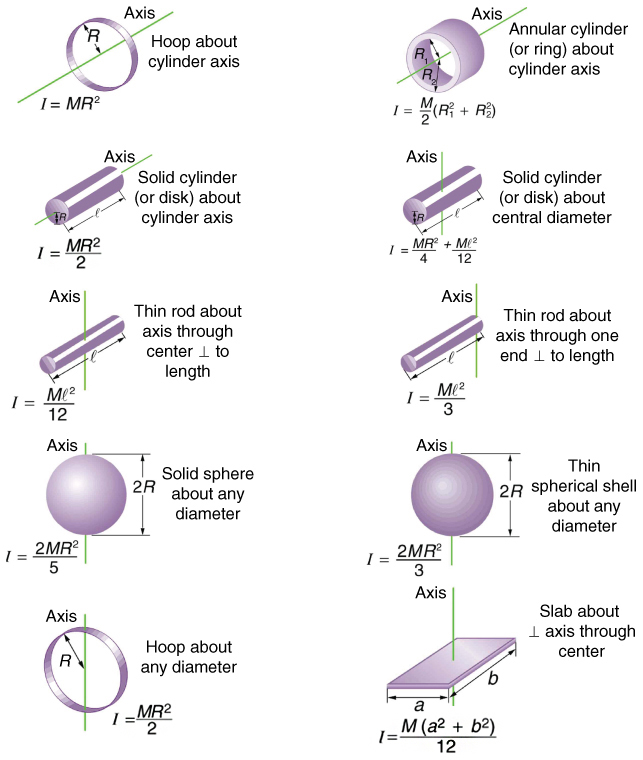
\includegraphics[height=8in,width=6in,angle=0]{moments.jpg}

\end{center}
 
 \section{Torque in Another Light}
 Torque may also be represented as the time rate of change of the angular momentum.
  $$\overrightarrow{\tau}\equiv \overrightarrow{r}\times  \overrightarrow{F}$$
  $$\overrightarrow{\tau}=\frac{d \overrightarrow{l}}{dt}$$
  
\section{Angular Momentum}
Angular momentum s a vector quantity that represents the product of a body's rotational inertia and rotational velocity about a particular axis. In the simple case of revolution of a particle in a circle about a center of rotation, the particle remaining always in the same plane and having always the same distance from the center, it is sufficient to discard the vector nature of angular momentum, and treat it as a scalar.  Angular momentum can be considered a rotational analog of linear momentum. Thus, where linear momentum is proportional to mass and linear speed angular momentum is proportional to moment of inertia and angular speed.

A single particle moves with an angular momentum $\overrightarrow{l}$.
 $$\overrightarrow{l}\equiv \overrightarrow{r}\times  \overrightarrow{p}$$
 \marginnote{The angular momentum, in general, only has meaning in reference to some center point.}
 $$\left|\overrightarrow{l}\right|= \left|\overrightarrow{r}\times  \overrightarrow{p}\right|=mr^2\omega$$
 The total angular momentum for a system of particles is notated $\overrightarrow{L}$.  It is calculated by the sum of the individual particle momenta.
  $$\overrightarrow{L}\equiv \sum_i \overrightarrow{l}_i $$
  Since each particle in a rigid body is moving at the same angular velocity we may represent the total angular momentum as the product of the moment of inertia and the angular velocity.
  \marginnote{The total angular momentum of a system is independent of the location of the reference point if the total linear momentum is equal to zero.  Can you prove that?  Can you choose a frame where the linear total momentum is equal to zero?  Do you see where we are going with this?}
  $$\overrightarrow{L}= \sum_i m_ir_i^2\omega$$
  $$\overrightarrow{L}= I\omega$$

\newpage
  
  \section{Conservation of Angular Momentum}
$$\overrightarrow{r}\times\overrightarrow{F}_{12}=-\overrightarrow{r}\times\overrightarrow{F}_{21}$$
\subsection{No External Torques}
\marginnote{This derivation is almost identical to that for conservation of linear momentum.}
$$\overrightarrow{r}\times\overrightarrow{F}_{2net}=-\overrightarrow{r}\times\overrightarrow{F}_{1net}$$
$$ \overrightarrow{r}\times\overrightarrow{F}_{2net}\ \Delta t=-\overrightarrow{r}\times\overrightarrow{F}_{1net}\ \Delta t$$
$$\Delta \overrightarrow{l}_{2}=-\Delta \overrightarrow{l}_{1}$$
$$\overrightarrow{l}_{2f} -\overrightarrow{l}_{2i}=-\overrightarrow{l}_{1f} +\overrightarrow{l}_{1i}$$
$$\overrightarrow{l}_{2f} +\overrightarrow{l}_{1f}=\overrightarrow{l}_{1i} +\overrightarrow{l}_{2i}$$
$$\overrightarrow{L}_{f}=\overrightarrow{L}_{i} $$
\subsection{External Forces}
\marginnote{If there are external torques they act to change the total angular momentum of the system.}
$$\sum{ \overrightarrow{\tau}_{ext}}=I\overrightarrow{\alpha}=\frac{\Delta\overrightarrow{L}}{\Delta t}$$
 


  \section{Rotational Work and Power}
  \marginnote{ The rotational analogue of work is the dot product between the torque and the angular displacement.  The net rotational work generates a change in rotational kinetic energy.  The time rate of change of the rotational work is the rotational power.}
 $$W_{rot}= \overrightarrow{\tau}\cdot \Delta \overrightarrow{\theta}$$
 $$P_{rot}=\lim_{\Delta\rightarrow 0}\frac{\Delta W_{rot}}{\Delta t}=\overrightarrow{\tau}\cdot \overrightarrow{\omega}$$

 
 \section{Rotational Kinetic Energy}
 $$\sum W_{rot}=\sum \overrightarrow{\tau}\cdot \Delta\overrightarrow{\theta}=\Delta KE_{rot}$$
 $$KE_{rot}=\frac{L^2}{2I}=\frac{I\omega^2}{2}$$
 $$KE=\underbar{KE}_{rot}+KE_{lin}=\frac{\underbar{L}^2}{2\underbar{I}}+\frac{\underbar{P}^2}{2M}=\frac{\underbar{I}\omega^2}{2}+\frac{Mv_{cm}^2}{2}$$

 \section{Rolling}
 \begin{marginfigure}[10pt]
  
\includegraphics[width=\linewidth]{rolling.jpg}
  \caption{This dog is rolling.}
  \label{fig:marginfig}
\end{marginfigure}
 $$v_{cm}=R\omega$$
 $$a_{cm}=R\alpha$$
 $$KE=\frac{I_p\omega^2}{2}=\frac{\underbar I}{2}\omega^2+\frac{MR^2}{2}\omega^2=\frac{1}{2}\left(\frac{\underbar I}{R^2}+M\right)v_{cm}^2$$
 \section{Precession of a Top}
  \section{Rolling}
 \begin{marginfigure}[10pt]
  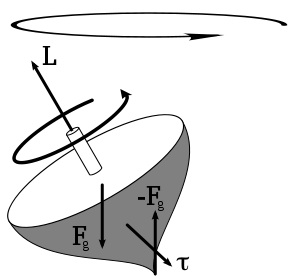
\includegraphics[width=\linewidth]{top.jpg}
  \caption{Precession of a top}
  \label{fig:marginfig}
\end{marginfigure}
 $$\sum{ \overrightarrow{F}_{ext}}=(F_n-Mg)\hat{z}=0$$
 $$\sum{ \overrightarrow{\tau}_{ext}}=\overrightarrow{0}\times(F_n\hat{z})+\overrightarrow{\scriptr}_{cm}\times(-Mg\hat{z})$$
 $$\frac{d\overrightarrow{L}}{dt}=-Mg\overrightarrow{\scriptr}_{cm}\times\hat{z}$$
 Precession is the result of the angular velocity of rotation and the angular velocity produced by the torque. It is an angular velocity about a line that makes an angle with the permanent rotation axis, and this angle lies in a plane at right angles to the plane of the couple producing the torque.  If the rotating body is symmetrical, its motion unconstrained and the torque on the spin axis is at right angles to that axis, the axis of precession will be perpendicular to both the spin axis and torque axis.
 \section{Quantization of Angular Momentum}
 Quantization of angular momentum is one of the deeper mysteries of the universe.  It was first postulated by Niels Bohr in his Bohr model of the atom and was later predicted by Erwin Schrodinger.  Angular momentum must be an integer multiple of the reduced Planck's constant $\hbar$.  The lowest possible angular momentum of a system is the reduced Planck's constant.
$$ L=n\hbar$$
$$ \underbar{I}\omega=n\hbar$$
$$ \hbar=\frac{h}{2\pi}=1.05\times 10^{-34}\  \footnotesize \frac{\text{kg}\cdot \text{m}^2}{\text{s}^2}$$




 